\documentclass[aspectratio=169]{beamer}

\usetheme{Madrid}
\usecolortheme{whale}
\setbeamertemplate{navigation symbols}{}
\setbeamertemplate{footline}[frame number]

\usepackage{graphicx}
\usepackage{booktabs}
\usepackage{amsmath}
\usepackage{siunitx}
\usepackage{xcolor}
\usepackage{tikz}

\definecolor{accent}{RGB}{0,102,153}
\definecolor{capsule}{RGB}{31,119,180}
\definecolor{deform}{RGB}{214,39,40}
\definecolor{highlight}{RGB}{0,153,76}

% Show a figure if it exists, else a "data pending" placeholder box.
% This lets the deck compile before the Isaac Sim runs are done.
\newcommand{\figordummy}[2]{%
  \IfFileExists{#1}{\includegraphics[width=#2\textwidth]{#1}}{%
    \fbox{\parbox[c][3cm][c]{#2\textwidth}{\centering\footnotesize
      \textcolor{gray}{[ figure pending ]}\\[2pt]
      \texttt{\detokenize{#1}}\\[2pt]
      run \texttt{run\_all.sh}}}}%
}

\title{Flexible Cable Simulation in NVIDIA Isaac Sim}
\subtitle{Rigid Capsule-Chain vs Deformable Body for Dual-Arm Manipulation}
\author{Ali Bani Asad}
\institute{University of Waterloo \\ Supervisor: Prof.\ Soo Jeon}
\date{\today}

\begin{document}

\begin{frame}
\titlepage
\end{frame}

\begin{frame}{Outline}
\tableofcontents
\end{frame}

% ====================================================================
\section{Problem Statement}
\begin{frame}{Problem Statement}
\begin{columns}[T]
\begin{column}{0.55\textwidth}
\begin{itemize}
    \item Isaac Sim \textbf{lacks native 1D deformable} support
    \item Need: realistic cable sim for \textbf{robotic manipulation}
    \item Two candidate models to evaluate:
    \begin{enumerate}
        \item \textcolor{capsule}{Rigid capsule-chain} (material-driven joints)
        \item \textcolor{deform}{FEM deformable body} (native soft-body)
    \end{enumerate}
\end{itemize}
\vspace{0.3cm}
\textbf{Material:} PUR (polyurethane) --- the most common\\
jacket for robot / drag-chain cables ($E \approx \SI{30}{MPa}$).
\vspace{0.2cm}

\textbf{Goal:} pick the best model for RL-based\\ cable manipulation.
\end{column}
\begin{column}{0.42\textwidth}
\centering
\figordummy{figures/two_robots_scene.pdf}{1.0}
\end{column}
\end{columns}
\end{frame}

% ====================================================================
\section{Method 1: Rigid Capsule-Chain}
\begin{frame}{Method 1: Rigid Capsule-Chain Model}
\begin{columns}[T]
\begin{column}{0.5\textwidth}
\textbf{Architecture:}
\begin{itemize}
    \item Chain of $N$ rigid capsules + D6 joints
    \item Bending: $K = EI/L_{\text{seg}}$ (beam theory)
    \item Axial MSD springs: $k_s = EA/L_{\text{seg}}$
    \item Twist DOF free (Govoni)
\end{itemize}
\vspace{0.3cm}
\textbf{Validated:} reproduces Govoni Table 1\\
stays stable where their explicit solver diverges\\
($800\times$ larger timestep).
\end{column}
\begin{column}{0.47\textwidth}
\centering
\figordummy{../cable_output/hanging_kick/frame_t5s.png}{1.0}\\
\small Hanging cable, 200 links, $E = \SI{30}{MPa}$
\end{column}
\end{columns}
\end{frame}

% ====================================================================
\section{Method 2: Deformable Body}
\begin{frame}{Method 2: FEM Deformable Body}
\begin{columns}[T]
\begin{column}{0.5\textwidth}
\textbf{Approach:}
\begin{itemize}
    \item Single deformable cylinder mesh
    \item FEM tetrahedral simulation
    \item Native self-collision + axial stretch
    \item Same PUR material ($E$, $\nu$, density)
    \item GPU-accelerated
\end{itemize}
\vspace{0.3cm}
\textbf{Setup:} \texttt{DeformableObjectCfg} +\\
\texttt{MeshCylinderCfg} +\\
\texttt{DeformableBodyMaterialCfg}
\end{column}
\begin{column}{0.47\textwidth}
\centering
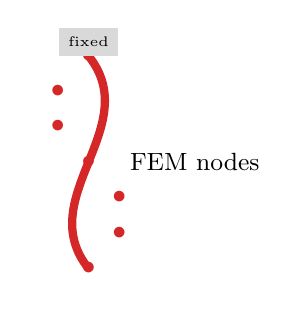
\begin{tikzpicture}[scale=0.9]
    \draw[deform, line width=3pt] (0,3) .. controls (0.8,2) and (-0.8,1) .. (0,0);
    \foreach \y in {0,0.5,1.0,1.5,2.0,2.5,3.0} {
        \node[deform] at ({0.5*sin(\y*120)},\y) {$\bullet$};
    }
    \node at (1.5,1.5) {\small FEM nodes};
    \node[fill=gray!30] at (0,3.2) {\tiny fixed};
\end{tikzpicture}\\
\small Continuous mesh, not discrete links
\end{column}
\end{columns}
\end{frame}

% ====================================================================
\section{Two-Robot Test}
\begin{frame}{Two-Robot Cable Manipulation Test}
\begin{columns}[T]
\begin{column}{0.46\textwidth}
\textbf{Setup:}
\begin{itemize}
    \item Two Franka Panda arms facing each other
    \item Each grasps one cable end
    \item Leader holds still
    \item Follower traces \SI{0.15}{m} sweep @ \SI{0.5}{Hz}
\end{itemize}
\vspace{0.3cm}
\textbf{We measure:}
\begin{itemize}
    \item Motion transmission (command vs response)
    \item Span error (inextensibility)
    \item Reaction force at follower
\end{itemize}
\end{column}
\begin{column}{0.52\textwidth}
\centering
\figordummy{figures/motion_transmission.pdf}{1.0}
\end{column}
\end{columns}
\end{frame}

% ====================================================================
\section{Comparison Criteria}
\begin{frame}{Comparison Criteria}
\centering
\small
\begin{tabular}{lcc}
\toprule
\textbf{Criterion} & \textbf{\textcolor{capsule}{Capsule-chain}} & \textbf{\textcolor{deform}{Deformable body}} \\
\midrule
Stability (dt = 1/240 s)   & Validated      & To test \\
Inextensibility            & Exact (rigid)  & Stretches (FEM) \\
Axial elasticity           & No             & Yes \\
Self-collision             & Approximate    & Native \\
Visual realism             & Good           & Excellent \\
Compute cost               & Low--moderate  & High \\
RL scalability             & High (many envs) & Low \\
\bottomrule
\end{tabular}

\vspace{0.5cm}
\begin{block}{Decision rule}
\textcolor{capsule}{Capsule-chain} for large-scale RL training (cheap, inextensible).\\
\textcolor{deform}{Deformable} for tasks needing knotting, wrapping, or force feedback.
\end{block}
\end{frame}

% ====================================================================
\begin{frame}{Comparison: Quantitative}
\begin{columns}[c]
\begin{column}{0.5\textwidth}
\centering
\figordummy{figures/span_error_compare.pdf}{1.0}\\
\small Inextensibility (span error)
\end{column}
\begin{column}{0.5\textwidth}
\centering
\figordummy{figures/compute_cost_compare.pdf}{1.0}\\
\small Force transmitted to follower arm
\end{column}
\end{columns}
\vspace{0.3cm}
\centering
\small All values measured from the two-robot Isaac Sim runs.
\end{frame}

% ====================================================================
\section{Next Steps}
\begin{frame}{Research Roadmap}
\centering
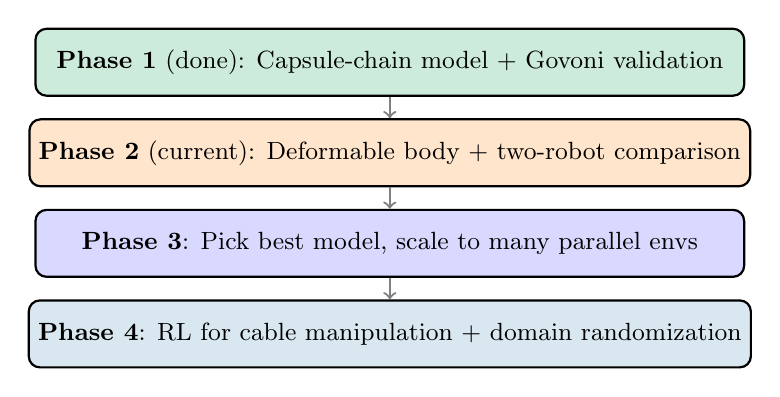
\begin{tikzpicture}[
    phase/.style={draw, thick, rounded corners, minimum width=9cm,
                  minimum height=0.85cm, align=center, font=\small},
    arr/.style={->, thick, gray},
]
    \node[phase, fill=highlight!20] (p1) at (0,4.0)
        {\textbf{Phase 1} (done): Capsule-chain model + Govoni validation};
    \node[phase, fill=orange!20] (p2) at (0,2.85)
        {\textbf{Phase 2} (current): Deformable body + two-robot comparison};
    \node[phase, fill=blue!15] (p3) at (0,1.7)
        {\textbf{Phase 3}: Pick best model, scale to many parallel envs};
    \node[phase, fill=accent!15] (p4) at (0,0.55)
        {\textbf{Phase 4}: RL for cable manipulation + domain randomization};
    \draw[arr] (p1) -- (p2);
    \draw[arr] (p2) -- (p3);
    \draw[arr] (p3) -- (p4);
\end{tikzpicture}
\vspace{0.3cm}

\textbf{RL background:} DDPG, TD3, SAC, PPO\\
\small Two published papers (ISA Transactions, Eng.\ Applications of AI)
\end{frame}

% ====================================================================
\section{Summary}
\begin{frame}{Summary}
\begin{enumerate}
    \item \textbf{Two cable models} built on common PUR material ($E = \SI{30}{MPa}$)
    \vspace{0.3cm}
    \item \textbf{Capsule-chain}: validated, cheap, inextensible --- RL-ready
    \vspace{0.3cm}
    \item \textbf{Deformable body}: physical stretch + self-collision --- higher fidelity
    \vspace{0.3cm}
    \item \textbf{Two-robot test} + criteria to choose between them objectively
    \vspace{0.3cm}
    \item \textbf{Next}: measured comparison $\rightarrow$ scale up $\rightarrow$ RL manipulation
\end{enumerate}
\vspace{0.4cm}
\centering
\textcolor{accent}{\textbf{Thank you. Questions?}}
\end{frame}

\begin{frame}[noframenumbering]{References}
\small
\begin{thebibliography}{9}
\bibitem{govoni2025} A.~Govoni et al.,
``Performance Analysis of a MSD DLO Model in Robotic Simulation Frameworks,''
\textit{arXiv:2504.13659}, 2025.
\bibitem{bergou2008} M.~Bergou et al.,
``Discrete Elastic Rods,'' \textit{ACM TOG (SIGGRAPH)}, 27(3), 2008.
\end{thebibliography}
\end{frame}

\end{document}
